%% Heatmap of the identified relationships between perceptions & conversation architecture

\begin{figure*}[t]
  \centering
  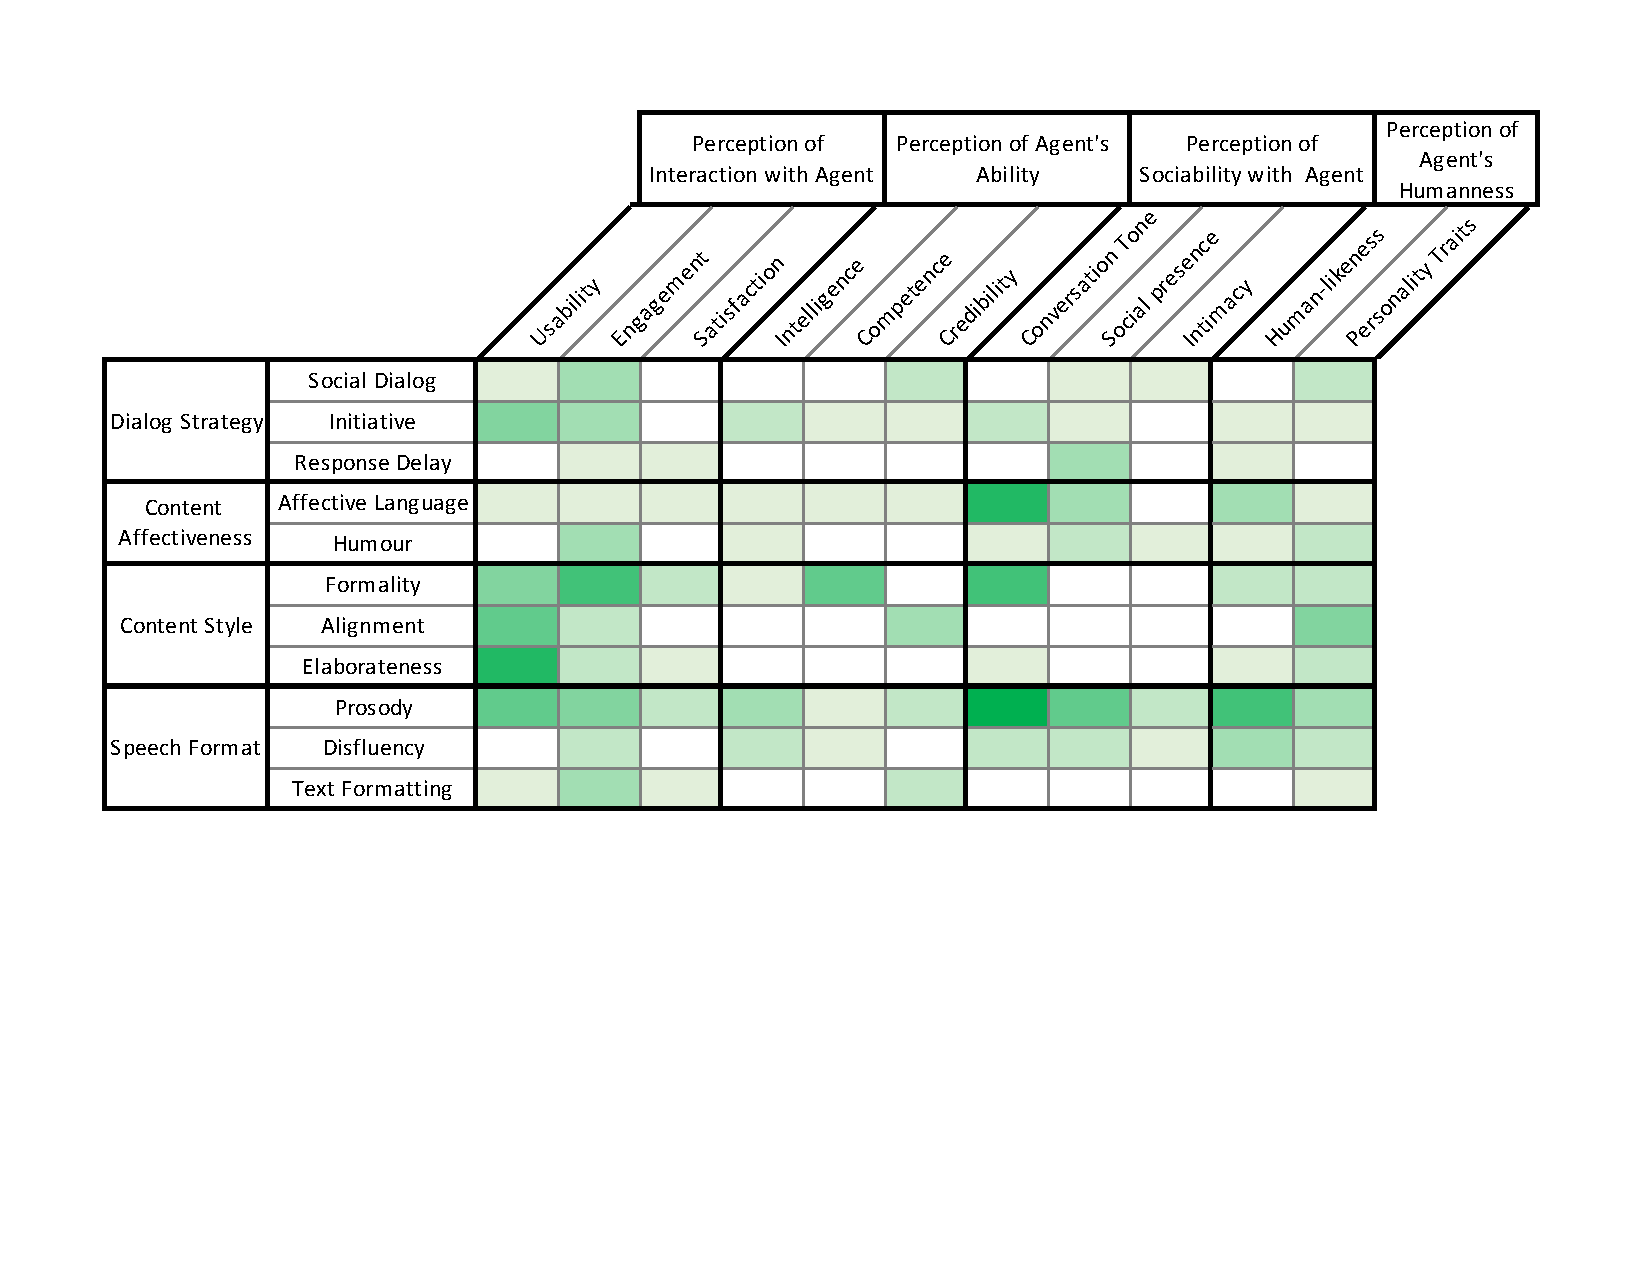
\includegraphics[width=0.9\textwidth]{figures/fig-heatmap_identified.pdf}
  \caption{Synthesized framework on the identified relationship between perception of agents and conversation architecture elements. The heatmap visualizes the number of relationships identified from the literature. Note that a single paper may describe more than one relationship.}
  \Description{This figure shows a heatmap the 183 identified relationships between conversation architecture elements and perceptions of agents. Each speech element is listed down the rows of the heatmap, grouped by the four categories dialog strategy, content affectiveness, content style, and speech format. Each perception aspect is listed across the columns of the table, grouped by the four categories perception of interaction with agent, perception of agent's ability, perception of sociability with agent, and perception of agent's humanness. Each cell has a different shade of colour, with the darker shades depicting higher number of relationships, and the lighter shades depicting smaller number of relationships.}
  \label{fig:heatmap_identified}
\end{figure*}